\chapter{Pro-sociality}
\label{chapter:pro-sociality}

In the previous chapter, one of the concluding remarks was the fact that humans tend to value the performance obtained by the team when they have robotic teammates. However, performance may sometimes be affected, or even damaged, by external factors, e.g., luck (such as in the card-game scenario). This consideration partially motivated our second research goal -- \textit{evaluate the impact of the team’s outcome on the collective cohesion} --, which we  discuss in the current chapter.

Additionally, we want to explore another dimension of cohesiveness, \textit{collective cohesion}. It reflects the degree of identification with the group. It is usually mentioned as the replacement of the ``I'' by the ``we'' and, when this feeling becomes stronger, it may even affect one’s actions with the collective goals taking priority over the individual ones. To investigate this question, we develop a new scenario where both the outcome could be controlled and the actions of the team members would express a degree of cooperation towards a collective goal. The scenario is called ``For The Record'', a collective risk dilemma mapped into an entertaining game, and its description is presented in Section~\ref{sec:for-the-record}.

We conducted a user study where a team constituted by two social robots and one person would play a session of ``For The Record'', as detailed in Section~\ref{sec:study3}. We manipulated not only the outcome of the game to either be a victory or a loss, but also the degree of cooperation on the two robots. This experimental set-up allowed us to investigate the following three research questions:
\begin{itemize}
    \item How do people perceive pro-social and selfish actions of robotic teammates?
    \item How can the perception of those robotic teammates be affected by the outcome of the team?
    \item Does the outcome of the team affect how humans identify with the team and trust it?
\end{itemize}

The chapter proceeds with the results of the user study in Section~\ref{sec:study3-results} and a detailed discussion of our hypotheses in Section~\ref{sec:study3-discussion}. Finally, some concluding remarks are presented in Section~\ref{sec:concluding-remarks}.

\section{For The Record}
\label{sec:for-the-record}
\textit{For The Record} is as a N-person threshold game with uncertain returns. In this game, there is a public good accessible by each team member independently of her contribution. The creation of such public good (their collective goal) requires that the sum of all contributions exceeds a threshold that is uncertain. Each player tries to maximise the collective goal by contributing to the public good. At the same time, individuals may opt to free ride on the efforts of others, while choosing to invest on their own individual goals. The game is set within an artistic context, in which players are musicians of a band. Even if framed within a specific context, this class of dilemmas is general enough to capture the non-linearity and uncertain nature of many Human collective endeavours, from group hunting to climate agreements. Introducing these type of social dilemmas in HRI, especially in group interactions, allows the analysis of pro-social collaboration and, in a more general perspective, the creation of new approaches in which robots can promote pro-sociality on humans.

The following description of \textit{For The Record} considers the artistic context attributed to the game when introduced to the players. Each musician of the band has the goal of ``maximising his/her revenue by contributing to the creation of successful albums and avoiding the collapse of the band''.

The game is composed by $R$ rounds and each round is the publication of an album on the market. Before detailing the stages of the album creation, consider that each player $j$ has two distinct skills as a musician that are quantifiable in discrete levels: the musical instrument ($li_j$), and the marketing ($lm_j$). 
The instrument skill is used during the creation of an album, where each player $j$ sequentially has to evaluate her individual performance by rolling $li_j$ dice of 6 faces. Letting $D_f(n)$ denote the result of rolling $n$ dice of $f$ faces, the value of an album sums the value of each musician's performance, according to the following expression:
\[ V_{album}=\sum_{i=1}^{N} D_6(li_j) \]
After creating each album, the market value determines whether that album succeeds or fails. The market value is calculated by rolling $n$ dice of 20 faces. Additionally, \textit{For The Record} includes two difficulty levels when publishing an album on the market, called national and international market that differ according to the following expressions:
\[V_{national\_market} = D_{20}(2)\]
\[V_{international\_market} = D_{20}(3)\]
Thereupon, each album is considered either a mega hit or a fail according to the following expression:
\[ \left\{ \begin{array}{ccl}
``Mega Hit'' & \mbox{if} & V_{album} >= V_{market}\\
``Fail'' & \mbox{if} & V_{album} < V_{market}
\end{array}\right.\]
Each round ends with the players receiving their individual revenues. The revenue is $0$ when the album has failed, however, in case of a mega hit, each player $j$ has two options: to receive a default amount of $3000$ or to use his/her marketing skill and receive according to the result of rolling $lm_j$ dice of 6 faces. This second option is only available if $lm_j > 0$.



%\begin{figure}[ht]
%    \centering
%    \includegraphics[width=0.8\columnwidth]{Images/forTheRecordMainGameplayScreenshot.png}
%    \caption{\tr{Interface of\textit{For The Record} at: (a) the level up phase, where each player chooses to upgrade the instrument (cooperate) or to upgrade the marketing (defect).}}
%    \label{fig:forTheRecordMainGameplayScreenshot}
%\end{figure}

In the beginning of each round, each player has to upgrade one of his/her skills by 1 point, between the instrument and the marketing skill. %\tr{(Figure~\ref{fig:forTheRecordMainGameplayScreenshot})}. 
On the one hand, by increasing the level of the instrument, the player can roll one more dice during the evaluation of his/her performance and, therefore, increases the likelihood of producing a successful album. On the other hand, by increasing the level of the marketing, the player can roll one more dice during the revenue collection in case of a mega hit and, therefore, increases the likelihood of maximising the individual profit. In other words, each player has to choose between to cooperate, by contributing to the collective goal, or to defect, by contributing to his/her individual goal.

Another important rule is: during the $R$ rounds, if the band achieves a limit $L$ of failed albums, the game ends and each musician loses all the accumulated revenue. This is done in order to stress the importance of collaborating.


\section{User Study}
\label{sec:study3}
We conducted a user study using the previously described \textit{For The Record} game. The number of players, $N$, was 3 and the selected setting was one human participant playing together with two robotic players on a touch screen (Figure~\ref{fig:interaction}).
Furthermore, we set the number of rounds, $R$, to 5 and the limit of failed albums, $L$, to 3. The band started to publish albums on the national market and changed to the international market on the $4^{th}$ round. The initial values for the levels of each skill were the same for all the players: 1 point in the instrument skill ($li=1$), and no points in the marketing skill ($lm=0$). Finally, players could upgrade their skills from the $2^{nd}$ round on, which means they had 4 decisions to make during the 5 rounds between improving their instrument skill (cooperate) or their marketing skill (defect).

\begin{figure}[ht]
    \centering
    \includegraphics[width=0.7\columnwidth]{images/prosociality/interaction1.png}
    \caption{This interaction was captured during a session of the user study, where a participant is playing \textit{For The Record} game with the two robotic partners.}
    \label{fig:interaction}
\end{figure}



One particular factor that is likely to influence how people perceive their robotic teammates is whether the team succeeds or fails in the shared task. As identified in \cite{kahneman2013choices}, people are more sensitive to avoiding losses than to gains of equal monetary amount. This well-known cognitive bias is referred to as loss aversion. As a result, in this user study, we manipulated the game result in a between-subjects design, which produced two experimental conditions: winning or losing the game. In order to achieve these two deterministic outcomes, we scripted predefined orders for all the possible dice throws. Not only could we guarantee all the participants played the same number of rounds, we could also ensure that the dice rolls of the each robot were the same in both conditions. Consequently, during the 5 rounds, participants got a failure, a victory, a failure, a victory and finally either a victory or a failure according to the condition.

The robotic players differ on the strategies they apply to play the game. One of them always defects by improving its marketing skill in every round, which we call the defector, while the other always cooperates by improving its instrument skill in every round, which we call the cooperator. Nevertheless, their verbal and non-verbal behaviours remained similar and we used two versions of the same embodiment for each character, the EMYS robotic head \cite{kkedzierski2013emys}. Regarding their speech acts, they encourage the team in the beginning of each album, they comment extreme luck or bad luck on the dice rolls for both themselves and the other players and, in the end of each album, they comment the round result with an emotional animation of either sadness or joy. The three game states that were used to emphasise the difference between their distinct game strategies were:
\begin{itemize}
    \item The level up phase where each robot chooses to upgrade either its instrument skill (cooperate) or its marketing skill (defect) (e.g., Cooperator -- ``I will level up the instrument.'', Defector -- ``I will improve the marketing.'');
    \item The dice roll that corresponds to the individual performance for an album (e.g., Cooperator -- ``Wow, I added [N] points!'', Defector -- ``[N] more points for our album!'');
    \item The last decision of using or not the marketing skill to receive the revenue in case of success (e.g., Cooperator -- ``Here it comes the reward.'', Defector -- ``I will use my [N] marketing skill points to see what I can get...'').
\end{itemize}
To avoid having these autonomous robots speaking at the same time, the game engine randomly chooses which robot comments each game state. Finally, their non-verbal behaviours consists of gazing at: the other players when it is their turn; the other robot if it is speaking; or the touch screen by default.



\subsection{Hypotheses}
The following hypotheses state our expectations towards the differences on people's perceptions, judgements and preferences between a pro-social and a selfish robotic partners after teaming with them in a public goods game.
\begin{itemize}
    \item[] \textbf{H1}: The pro-social robot will be perceived more positively in its social attributes than the selfish robot.
    \item[] \textbf{H2}: The pro-social robot will be perceived as less competent than the selfish robot.
    \item[] \textbf{H3}: Group trust and group identification will be positively associated with the group performance.
    \item[] \textbf{H4}: When the team wins, the main responsible factor will be the strategy of the pro-social robot.
    \item[] \textbf{H5}: When the team loses, the main responsible factor will be the strategy of the selfish robot.
    \item[] \textbf{H6}: The pro-social robot will be preferred as a future partner, rather than the selfish robot.
\end{itemize}

Our rationale behind these hypotheses is the following. Concerning \textbf{H1} and \textbf{H6}, we expect that participants see the pro-social robot in a more positive light as it acts in a fully collaborative manner, helping the team to succeed.
The expectation behind \textbf{H2} lies in the fact that the selfish robot will always be ahead in terms of task performance (profit made). Additionally, in a study that asked participants to judge the competence of people playing the prisoner's dilemma, the results showed that those who were defected against were seen as less competent \cite{krueger2007perceptions}. It is possible that the same effect occurs in our study given that pro-social robot's behaviour. The reason for \textbf{H3} is the aforementioned loss aversion bias \cite{kahneman2013choices} and finally, \textbf{H4} and \textbf{H5} are based on the assumption that people will correctly identify the main responsible actor behind the team's result.

\subsection{Procedure}
Participation in this study was individual and started with a brief overview of each step. All the participants signed the consent form and then proceeded with the experiment. One researcher read the game rules one by one and answered participant's questions, while another researcher set up the robots and the video camera. Then, they played a training game without the robots to ensure the participant learned the game and to clarify any final doubts. The training game had a maximum of 5 rounds but the dice rolls were completely random. After that, the researcher initiated the game with the robots, alternating between conditions. Before the researchers left the room, they emphasised the goal of the study is to analyse their opinion of each robot and, therefore, they should pay attention to which is which and also to their behaviours during the game. Finally, after the interaction with the robots, each participant answered the questionnaire and was greeted by his/her participation.


\subsection{Dependent Measures}
The following dependent measures were used on the data analysis: \textbf{Competitiveness} level of the participant using a single-item question ``How competitive do you evaluate yourself?''; \textbf{Group Identification} \cite{leach2008group} using the Portuguese adaptation \cite{ramos2011adaptaccao} with the dimensions of Solidarity, Satisfaction and In-Group Homogeneity; \textbf{Group Trust} \cite{allen2004exploring}; \textbf{RoSAS} \cite{carpinella2017robotic} using its three dimensions of Warmth, Discomfort, and Competence towards each robot; \textbf{Choice of a Robotic Partner} among the defector and the cooperator for a hypothetical future game; \textbf{Responsibility (blame/credit) attribution} of four different factors -- randomness, participant's strategy, defector's strategy and cooperator's strategy -- using single-item questions ``The game result was mainly due to (...)''.
All the items in the questionnaire were assessed in a 7-points scale ranging from 1 (``Definitely not associated'') to 7 (``Definitely associated'') and the robots were always mentioned by their names.

\subsection{Sample}
The study was conducted at a company facility in order to collect a varied sample in terms of age, gender and background. There was a total of 70 participants (35 per experimental condition) with ages ranging from 22 to 63 ($M=34.6, SD=11.557$). Regarding gender, there were 32 females, 37 male, and 1 unknown.


\section{Results}
\label{sec:study3-results}
\subsection{Social Attributes of the Robots}
%\label{sec:rosas}
To analyse the impact of the game result on the perception of each robot, we used a Mixed analysis of variance (ANOVA) where the within-subjects factor is the robotic character and the between-subjects factor is the game result (winning or losing).

Regarding the perception of warmth, there was a significant main effect of the robotic character (Figure~\ref{fig:main-effects}, $F(1,67)=17.366, p<0.001, r=0.454$) with the cooperator being rated with higher values of warmth ($M=4.225, SD=1.090$) compared to the defector ($M=3.513, SD=0.977$). However, the main effect of the game result and the interaction between the robotic character and the game result were not statistically significant ($F(1,67)=0.028, p=0.869, r=0.020$ and $F(1,67)=0.013, p=0.908, r=0.014$, respectively).

For the social attribute of discomfort, there was a main effect of the robotic character (Figure~\ref{fig:main-effects}, $F(1,67)=30.982, p<0.001, r=0.562$), with the defector being rated with higher levels of discomfort ($M=2.895, SD=1.302$) than the cooperator ($M=1.895, SD=1.064$). Again, we have not found a significant main effect of the game result nor a significant interaction between the robotic character and the game result ($F(1,67)=0.525, p=0.471, r=0.088$ and $F(1,67)=1.141, p=0.289, r=0.129$, respectively).


\begin{figure}[ht]
\centering
%%% PLOT FILE - Perceptions of the robots - main effect of the robot on warmth and discomfort
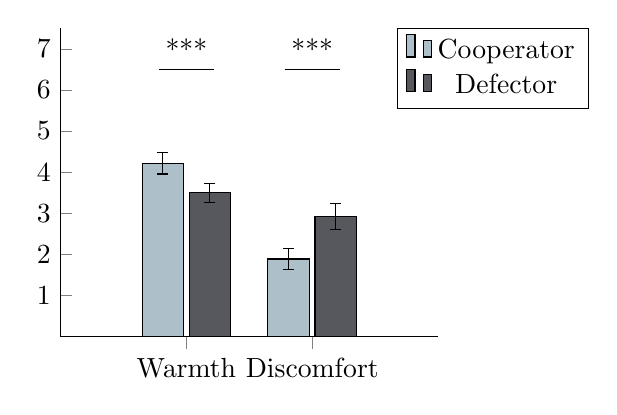
\begin{tikzpicture}%
\begin{axis}[%
    ybar,%
    %title=Test,%
    axis y line*=left, axis x line*=bottom,%
    ymin=0,
    ymax=7.5,
    ytick={1,2,...,7},
    legend style={at={(1.4,1)}},
    %x tick label style={rotate=45,anchor=east},%
    symbolic x coords={Warmth,Discomfort},%
    xtick=data,
    enlarge x limits=1,
    bar width=15pt,
    height=5.5cm,
    %ylabel=difference in \%,%
        ]%
\addplot+[
    color=black, %
    fill={rgb,255:red,173; green,192; blue,202},%
    %postaction={pattern=crosshatch dots},
    error bars, y dir=both, y explicit]
				coordinates {
				(Warmth,4.22) +- (Warmth,0.264)
				(Discomfort,1.89) +- (Discomfort,0.258)};
\addplot+[%
    color=black, %
    fill={rgb,255:red,87; green,87; blue,94},%
    error bars/.cd,%
    y dir=both,%
    y explicit,%
        ]%
coordinates {
            (Warmth,3.50) +- (Warmth,0.236)
            (Discomfort,2.92) +- (Discomfort,0.31)
        };%
    
\draw (axis cs:Warmth,6.5) ++ (-10pt,0pt) -- ++(20pt,0pt);
\node[anchor=south] at (axis cs:Warmth,6.5) {***};
    
\draw (axis cs:Discomfort,6.5) ++ (-10pt,0pt) -- ++(20pt,0pt);
\node[anchor=south] at (axis cs:Discomfort,6.5) {***};

\legend{Cooperator,Defector}
\end{axis}%
\end{tikzpicture}%
\caption{Main effect of the robotic partner on the social attributes of warmth and discomfort.}
\label{fig:main-effects}
\end{figure}

These results suggest that the distinct strategies adopted by the robots affected the perception of the robot's warmth and the discomfort they felt regardless of the game result.

In terms of the perception of competence, there was a significant main effect of the robotic character ($F(1,67)=24.873, p<0.001, r=0.520$), with the the cooperator being rated with higher levels of competence ($M=4.790, SD=1.111$) than the defector ($M=3.907, SD=1.073$). Although we did not find a significant effect of the game result ($F(1,67)=0.966, p=0.329, r=0.119$), there was a significant interaction between the robotic character and the game result (Figure~\ref{fig:interaction-effect}, $F(1,67)=4.095, p=0.047, r=0.240$). To understand this interaction, we compared the perception of competence attributed to each robot across the two possible game results using a Wilcoxon Signed-Rank test. In the case where the game result was winning, there was no significant difference between the competence attributed to each robot ($Z=-1.859, p=0.063, r=-0.319$). However, in the case where the game result was losing, there was a significant difference between the competence attributed to each robot ($Z=-4.434, p<0.001, r=-0.749$), with the cooperator being rated as more competent ($M=4.876, SD=0.958$) than the defector ($M=3.624, SD=0.896$).


\begin{figure}[ht]
\centering
%%% PLOT FILE - Perceptions of the robots - interaction effect on competence between robot and condition
\begin{tikzpicture}%
\begin{axis}[%
    %ybar,%
    %title=Test,%
    axis y line*=left, axis x line*=bottom,%
    ymin=0,
    ymax=7.5,
    ytick={1,2,...,7},
    legend style={at={(1.4,1)}},
    %x tick label style={rotate=45,anchor=east},%
    symbolic x coords={Winning,Losing},%
    xtick=data,
    enlarge x limits=1,
    bar width=15pt,
    height=5.5cm,
    %ylabel=difference in \%,%
        ]%
\addplot+[
    color=black, %
    %mark size=4pt,
    mark options={
    fill={rgb,255:red,173; green,192; blue,202},%
    },
    error bars, y dir=both, y explicit]
				coordinates {
				(Winning,4.70) +- (Winning,0.382)
				(Losing,4.88) +- (Losing,0.376)};
\addplot+[%
    color=black, %
    mark size=2pt,
    mark options={
    fill={rgb,255:red,87; green,87; blue,94},%
    },
    error bars/.cd,%
    y dir=both,%
    y explicit,%
        ]%
coordinates {
            (Winning,4.17) +- (Winning,0.358)
            (Losing,3.62) +- (Losing,0.353)
        };%


\draw (axis cs:Losing,4.25) ++ (10pt,-10pt) -- ++(0pt,20pt);
\node[anchor=south] at (140,380) {***};

%\draw (axis cs:Winning,4.4) ++ (-10pt,-10pt) -- ++(0pt,20pt);
%\node[anchor=south] at (-30,410) {n.s.};

\legend{Cooperator,Defector}
\end{axis}%
\end{tikzpicture}%
\caption{Interaction effect between the robotic partner and game result on the attributed levels of competence.}
\label{fig:interaction-effect}
\end{figure}

Contrary to the previous social attributes, the competence attributed to each robot was affected by the game result. Participants have considered the cooperator as more competent only in the losing condition. This result suggests the negative effect of losing the game highlighted the difference in perceived competence between the robots.

\subsection{Group Measures}

To analyse the two dependent measures related to the group (Figure~\ref{fig:group}), i.e. group identification and group trust, between the two possible game results, we used Mann-Whitney U tests. Results showed a significant difference between the levels of group identification according to the condition ($U=404.5, Z=-2.445, p=0.014, r=-0.292$), with participants that won the game reporting higher levels of group identification ($M=4.267, SD=1.346$) than participants who have lost the game ($M=3.466, SD=1.182$). Nevertheless, there was no significant difference between the levels of group trust according to the game result ($U=535.5, Z=-0.715, p=0.474, r=-0.086$).


\begin{figure}[ht]
\centering
%%% PLOT FILE - Group measures condition
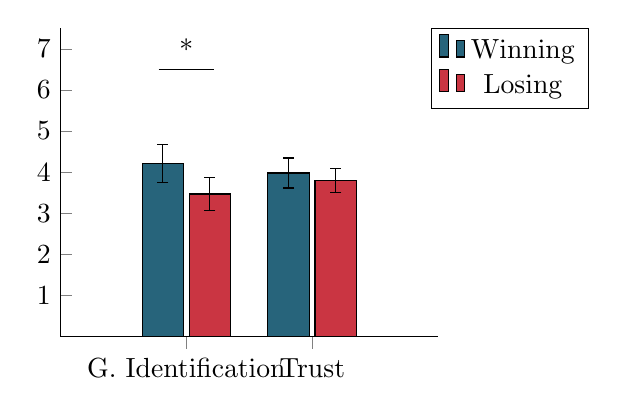
\begin{tikzpicture}%
\begin{axis}[%
    ybar,
    %title=Test,%
    axis y line*=left, axis x line*=bottom,%
    ymin=0,
    ymax=7.5,
    ytick={1,2,...,7},
    legend style={at={(1.4,1)}},
    %x tick label style={rotate=45,anchor=east},%
    symbolic x coords={G. Identification,Trust},%
    xtick=data,
    enlarge x limits=1,
    bar width=15pt,
    height=5.5cm,
    %ylabel=difference in \%,%
        ]%
\addplot+[%
    color=black, %
    fill={rgb,255:red,39; green,100; blue,123},%
    %postaction={pattern= north east lines},
    error bars/.cd,%
    y dir=both,%
    y explicit,%
        ]%
coordinates {
            (G. Identification,4.22) +- (G. Identification,0.464)
            (Trust,3.98) +- (Trust,0.365)
        };%
\addplot+[
    color=black,
    fill={rgb,255:red,202; green,53; blue,66},%
    error bars, y dir=both, y explicit]
				coordinates {
				(G. Identification,3.47) +- (G. Identification,0.407)
				(Trust,3.79) +- (Trust,0.291)};
    
\draw (axis cs:G. Identification,6.5) ++ (-10pt,0pt) -- ++(20pt,0pt);
\node[anchor=south] at (axis cs:G. Identification,6.5) {*};

\legend{Winning,Losing}
\end{axis}%
\end{tikzpicture}%
\caption{Effect of the game result on the attributed levels of group identification and group trust.}
\label{fig:group}
\end{figure}

These results revealed the group identification was affected by the game result, winning or losing the game, as we have predicted. However, the prediction about the measure of group trust was not confirmed, suggesting that other factors might have contributed to this outcome. Therefore, we conducted an additional analysis to interpret these surprising findings, by creating predictive models of both the group identification and the group trust levels. We used Stepwise regressions with the backward method to determine which variables could explain most of the variance of group identification and group trust levels. The initial seven predictor variables were the ones related with individual and group perceptions of the team members: defector's warmth, defector's competence, defector's discomfort, cooperator's warmth, cooperator's competence, cooperator's discomfort, and either group identification or group trust.

Regarding the group identification level, % (Table~\ref{tab:group-id-reg}), 
we found in the $5^{th}$ step that it can be significantly predicted ($F(3,65)=33.016, p<0.001, R^2=0.604$) by - $1.652$ + $0.843$ (group trust) + $0.375$ (defector's competence) + $0.158$ (cooperator's competence), where variables are assessed with 7-points likert scales. %The remaining possible predictors were excluded according to the removal criterion of not making a significant contribution to the model, respectively: defector's warmth ($t(2)=-0.179, p=0.859$) in $1^{st}$ step ($F(7,61)=14.294, p<0.001, R^2=0.621$); cooperator's warmth ($t(2)=0.252, p=0.802$) in $2^{nd}$ step ($F(6,62)=16.935, p<0.001, R^2=0.621$); defector's discomfort ($t(2)=0.475, p=0.636$) in $3^{rd}$ step ($F(5,63)=20.616, p<0.001, R^2=0.621$); and cooperator's discomfort ($t(2)=1.332, p=0.188$) in $4^{th}$ step ($F(4,64)=26.028, p<0.001, R^2=0.619$).
%\begin{table}[ht]
%\centering
%\renewcommand{\arraystretch}{1.2}
%\begin{tabular}{lccc}
 %                   & \textbf{B} & \textbf{SE B} & \textbf{$\beta$} \\ \hline
%Constant            & -1.721     & 0.673         &                  \\
%Group Trust         & 0.849      & 0.114         & 0.610            \\
%Defector's Competence   & 0.391      & 0.101         & 0.318            \\
%Cooperator's Competence & 0.159      & 0.093         & 0.134           
%\end{tabular}
%\caption{Predictive model of the group identification level at the $5^{th}$ step using the forward method.}\label{tab:group-id-reg}
%\end{table}
Regarding the prediction of the group trust level, % (Table~\ref{tab:group-trust-reg}), 
we found in the $6^{th}$ step that it can be significantly predicted ($F(2,66)=40.455, p<0.001, R^2=0.551$) by $2.513$ + $0.489$ (group identification) - $0.174$ (defector's discomfort), where variables are assessed with 7-points likert scales. %The remaining variables were excluded according to the removal criterion of not making a significant contribution to the model, respectively: defector's warmth ($t(2)=0.764, p=0.448$) in $1^{st}$ step ($F(7,61)=11.284, p<0.001, R^2=0.564$); cooperator's warmth ($t(2)=0.666, p=0.508$) in $2^{nd}$ step ($F(6,62)=13.207, p<0.001, R^2=0.561$); cooperator's discomfort ($t(2)=-0.769, p=0.445$) in $3^{rd}$ step ($F(5,63)=15.900, p<0.001, R^2=0.558$); cooperator's competence ($t(2)=-0.447, p=0.657$) in $4^{th}$ step ($F(4,64)=19.854, p<0.001, R^2=0.554$); and defector's competence ($t(2)=-1.204, p=0.233$) in $5^{th}$ step ($F(3,65)=26.735, p<0.001, R^2=0.552$).

%\begin{table}[ht]
%\centering
%\renewcommand{\arraystretch}{1.2}
%\begin{tabular}{lccc}
%                    & \textbf{B} & \textbf{SE B} & \textbf{$\beta$} \\ \hline
%Constant            & 2.487     & 0.326         &                  \\
%Group Identification         & 0.481      & 0.061         & 0.669            \\
%Defector's Discomfort & -0.160      & 0.061         & -0.220           
%\end{tabular}
%\caption{Predictive model of the group trust level at the $6^{th}$ step using the forward method.}\label{tab:group-trust-reg}
%\end{table}

This exploratory analysis allowed us to understand that although there is a correlation between group identification and group trust, they were affected by other factors, after partialling out the shared explanatory effect of the other variables. Besides the strong relation of one another, group identification can also be predicted from the competence attributed to each of the team members, and group trust can also be predicted from the discomfort attributed to the defector.

\subsection{Responsibility (Blame / Credit) Attribution}

To analyse the responsibility attribution of the game result among the following four factors of (1) randomness, (2) participant's strategy, (3) defector's strategy and (4) cooperator's strategy, we used Friedman's ANOVA tests. In the winning condition (Figure~\ref{fig:credit}), we found no significant differences on the credit attribution to the four factors ($\chi^2(3)=7.142, p=0.067, r=0.070$). However, in the losing condition (Figure~\ref{fig:blame}), the blame attribution was significantly different to the four possible factors ($\chi^2(3)=33.264, p<0.001, r=0.326$).



\begin{figure}[ht]
\centering
%%% PLOT FILE - Responsibility attribution in the winning condition
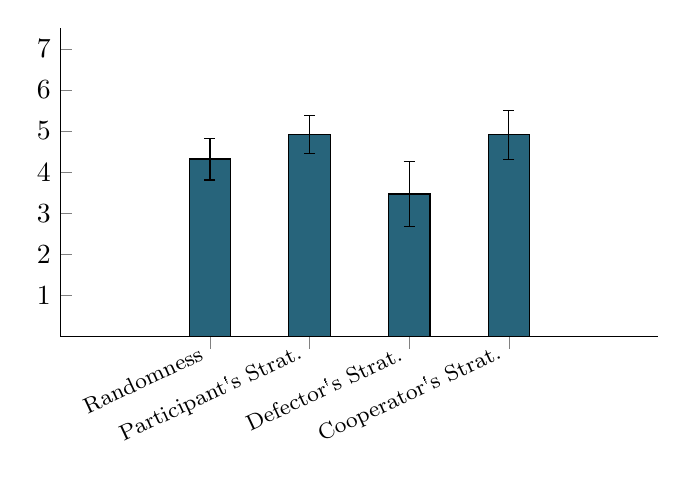
\begin{tikzpicture}%
\begin{axis}[%
    ybar,
    %title=Test,%
    axis y line*=left, axis x line*=bottom,%
    ymin=0,
    ymax=7.5,
    ytick={1,2,...,7},
    %legend style={at={(1.4,1)}},
    x tick label style={rotate=25,anchor=east},
    symbolic x coords={Randomness,Participant\textquotesingle s Strat.,Defector\textquotesingle s Strat.,Cooperator\textquotesingle s Strat.},%
    xtick=data,
    x=36pt,
    enlarge x limits=0.5,
    height=5.5cm,
    bar width=15pt,
    xticklabel style={font=\footnotesize},]%
\addplot+[
    color=black,
    fill={rgb,255:red,39; green,100; blue,123},%
    %postaction={pattern= north east lines},
    error bars, y dir=both, y explicit]
				coordinates {
				(Randomness,4.32) +- (Randomness,0.51)
				(Participant\textquotesingle s Strat.,4.91) +- (Participant\textquotesingle s Strat.,0.46)
				(Defector\textquotesingle s Strat.,3.47) +- (Defector\textquotesingle s Strat.,0.78)
				(Cooperator\textquotesingle s Strat.,4.91) +- (Cooperator\textquotesingle s Strat.,0.6)};
%\legend{Winning,Losing}
\end{axis}%
\end{tikzpicture}%
\caption{Responsibility attributed to each factor in winning condition (credit).}
\label{fig:credit}
\end{figure}

\begin{figure}[ht]
\centering
%%% PLOT FILE - Responsibility attribution in the losing condition
\begin{tikzpicture}%
\begin{axis}[%
    ybar,
    %title=Test,%
    axis y line*=left, axis x line*=bottom,%
    ymin=0,
    ymax=7.5,
    ytick={1,2,...,7},
    %legend style={at={(1.4,1)}},
    x tick label style={rotate=25,anchor=east},%
    symbolic x coords={Randomness,Participant's Strat.,Defector's Strat.,Cooperator's Strat.},%
    xtick=data,
    x=36pt,
    enlarge x limits=0.5,
    height=5.5cm,
    bar width=15pt,
    xticklabel style={font=\footnotesize}
    %ylabel=difference in \%,%
        ]%
\addplot+[
    color=black,
    fill={rgb,255:red,202; green,53; blue,66},%
    error bars, y dir=both, y explicit]
				coordinates {
				(Randomness,3.50) +- (Randomness,0.58)
				(Participant's Strat.,3.26) +- (Participant's Strat. Strat.,0.49)
				(Defector's Strat.,5.56) +- (Defector's Strat.,0.53)
				(Cooperator's Strat.,3.26) +- (Cooperator's Strat.,0.59)};
    
\addplot[black, sharp plot]%
    coordinates {(Participant's Strat.,6.3) (Defector's Strat.,6.3)}%
    node[above] at (150,610) {*};%
\addplot[black, sharp plot]%
    coordinates {(Defector's Strat.,6.6) (Cooperator's Strat.,6.6)}%
    node[above] at (250,640) {*};%
\addplot[black, sharp plot]%
    coordinates {(Randomness,6.9) (Defector's Strat.,6.9)}%
    node[above] at (100,670) {*};%
%\draw (axis cs:Participant's Strat.,6.5) ++ (-10pt,0pt) -- ++(20pt,0pt);
%\node[anchor=south] at (axis cs:Participant's Strat.,6.5) {***};
\end{axis}%
\end{tikzpicture}%
\caption{Responsibility attributed to each factor in losing condition (blame).}
\label{fig:blame}
\end{figure}


To follow up this finding on the attribution of blame, we conducted a \textit{post hoc} analysis using Wilcoxon Ranks tests. Moreover, we applied a Bonferroni correction and all the effects are reported at a $0.008$ level of significance. It appeared that all the pairwise comparisons involving the defector's strategy were significant. In the losing condition, participants attributed higher levels of blame to the defector's strategy ($M=5.429, SD=1.685$) when compared to the randomness factor ($M=3.543, SD=1.669; Z=-3.421, p<0.001, r=-0.578$), to the participant's strategy ($M= 3.265, SD=1.377; Z=-4.586, p<0.001, r=-0.786$), and to the cooperator's strategy ($M= 2.743, SD=1.669; Z=-3.909, p<0.001, r=-0.661$). Regarding the remaining pairwise comparisons, there was no significant difference between levels of blame attributed to the randomness factor and to the participant's strategy ($Z=-0.745, p=0.456, r=-0.128$), nor between the randomness factor and the cooperator's strategy ($Z=-2.201, p=0.028, r=-0.372$), nor between the participant's strategy and the cooperator's strategy ($Z=-1.284, p=0.199, r=-0.220$). These results reveal that there was no clear main responsible factor in the credit attribution of the winning outcome. However, participants clearly identified the defector's strategy as the main cause of the losing outcome.


\subsection{Choice of a Robotic Partner}

To analyse the choice of a robotic partner among the defector and the cooperator for a hypothetical future game, we used a Chi-Square Goodness-of-Fit test. Results indicated a significant difference in the preference for a robotic partner ($\chi^2(1)=22.857, p<0.001, r=0.326$), with the cooperator being preferred (55 times, $78.6$\%) to the defector (15 times, $21.4$\%).

Additionally, we found a significant association between the preferred robot and the game result ($\chi^2(1)=14.339, p<0.001, \phi_c=0.453$) and we have, therefore, also analysed preferences across conditions (Figure~\ref{fig:preferences}). In the losing condition, there was again a significant difference ($\chi^2(1)=31.114, p<0.001, r=0.889$), with the cooperator being preferred (34 times, $97.1$\%) to the defector (1 time, $2.9$\%). However, in the winning condition, no significant difference was found ($\chi^2(1)=1.400, p=0.237, r=0.040$), with the cooperator being chosen 21 times ($60.0$\%) and the defector 14 times ($40.0$\%).


\begin{figure}[ht]
\centering
%%% PLOT FILE - Choice of a robotic partner
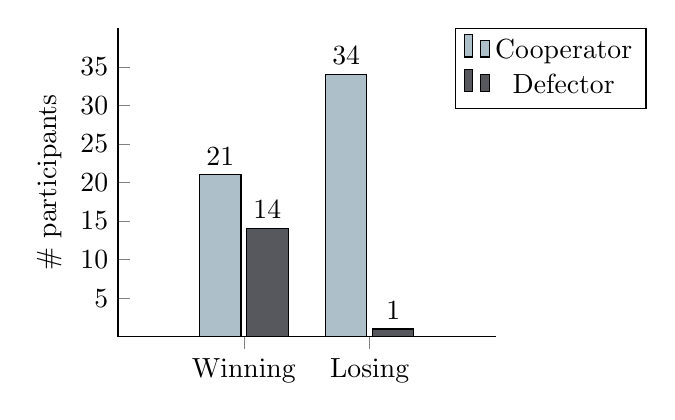
\begin{tikzpicture}%
\begin{axis}[%
    ybar,
    %title=Test,%
    axis y line*=left, axis x line*=bottom,%
    ymin=0,
    ymax=40,
    ytick={5,10,...,35},
    legend style={at={(1.4,1)}},
    %x tick label style={rotate=45,anchor=east},%
    symbolic x coords={Winning, Losing},%
    xtick=data,
    enlarge x limits=1,
    height=5.5cm,
    bar width=15pt,
    ylabel=\# participants,%
    nodes near coords,
        ]%
\addplot+[
    color=black, %
    fill={rgb,255:red,173; green,192; blue,202},%
    %postaction={pattern=crosshatch dots},
    %error bars,
    y dir=normal,
    %y explicit
    ]
				coordinates {
            (Winning,21.0)
            (Losing,34.0)
				};
\addplot+[%
    color=black, %
    fill={rgb,255:red,87; green,87; blue,94},%
    %error bars/.cd,%
    y dir=normal,%
    %y explicit,%
        ]%
coordinates {
            (Winning,14.0)
            (Losing,1.0)
        };%
\legend{Cooperator,Defector}
\end{axis}%
\end{tikzpicture}%
\caption{Preferences for each robotic partner grouped by conditions.}
\label{fig:preferences}
\end{figure}

When breaking down the choices of the participants across conditions, their preference is only clear when they lost the game. These results suggest that the negative impact of losing the game enhances the selfishness of the defector.


%\subsection{Strategies and Impressions of the Participants}
\subsection{Strategy analysis}
We analysed the playing strategies of the participants by looking at the number of times they have defected among their 4 decisions during the game. There were 8 participants that have never defected (11.4\%), 21 that have defected once (30\%), 33 that have defected twice (47.1\%), 7 that have defected 3 times (10\%), and only 1 that always defected (1.4\%). Furthermore, out of the 33 that defected 2 times, 24 of them chose the strategy of ``cooperate, defect, cooperate, and defect''. Additionally, we found a weak positive correlation between the self-reported competitiveness level of the participants and the number of times they have defected ($r(70)=0.235, p=0.05$).

%\tmightremove{Although the profit each robot achieved during the game was scripted, the profit of the participant varies according to his decisions. We analysed the differences between the average profit that each player got, considering for the losing condition the values they have accumulated until the $4^{th}$ round. Using Friedman's ANOVA test, we found there is a significant difference between the profit of each player ($\chi^2(2)=124.427, p<0.001, r=0.889$). Moreover, all the pairwise comparisons revealed significant differences: between the profit of the defector ($M=25.000, SD=9.065$) and the profit of the participants ($Z=-7.300, p<0.001, r=-0.872; M=10.329, SD=4.442$); between the profit of the cooperator ($M=7.500, SD=1.511$) and profit of the participant ($Z=-6.104, p<0.001, r=-0.730$); and between the profit of the defector and the profit of the cooperator ($Z=-7.504, p<0.001, r=-0.897$). In other words, the pro-social robot had less profit than the others, the selfish robot had more profit than the others, and the participant had an in-between average profit.}

Finally, we did a correlation analysis to understand if the participants' perceptions of the robotic partners were associated with their competitiveness level or their playing strategy. In the winning condition, we found a moderate negative correlation between the rate of cooperation and the perceived impact of the defector’s strategy ($r=-0.379, n=34, p=0.027$) and a moderate positive correlation between the rate of cooperation and the perceived impact of the self strategy ($r=0.426, n=35, p=0.011$). No similar significant correlations were found in the losing condition. This suggests participants that cooperated more with team attributed more credit to their own strategy and less credit to the defector's strategy.

\subsection{Societal Impact}
Due to the diversity of our sample, we asked participants, at the end of the questionnaire, their agreement level on the sentence ``Social robots will be relevant to the society'', ranging between 1 (``Totally disagree'') and 7 (``Totally agree'').
Interestingly, we found a significant difference on their answers between conditions ($U=435, Z=-2.143, p=0.032, r=-0.256$), revealing a higher acceptance of social robots when they won the game ($M=5.457, SD=1.651$), compared to when they lost the game ($M=4.686, SD=1.676$).



\section{Discussion}
\label{sec:study3-discussion}
According to \textbf{H1}, we have predicted that the pro-social robot would be perceived more positively than the selfish robot. We validated this hypothesis as the cooperator was rated as warmer and caused less discomfort. Our results suggest that the display of a pro-social strategy by the robotic partner enhanced the perception of its social attributes.

We have also predicted in \textbf{H2} that the selfish robot would be perceived as more competent, which was not confirmed. In fact, the opposite result was found, although only in the losing condition. This hypothesis was based on the fact that the defector uses the optimal strategy of maximising its profit on the efforts of the others, commonly called the free rider. One possible explanation is that participants construed the notion of competence as one that necessitates the absence of exploitation of others and, therefore, even though selfish acts are highly profitable, they are deemed as incompetent. It is also the case that, in the long run with multiple iterations of the game being played, the higher return obtained by a selfish strategy will diminish when considering the results obtained for the future partner choice in the losing condition. Another possible contributing factor is that participants were highly sensitive to the risk involved in the uncertainty threshold of this game. Consequently, when participants lost the game, the evidence of a risky strategy became blameworthy and unreasonable.

Our results partially support \textbf{H3} as group identification was indeed positively associated with the performance of the group, although the same association was not verified for group trust. This surprising difference led us to analyse more carefully which factors were predicting both measures. According to our regression analysis, the best predictors of group identification were the group trust and the competence of each team member. Considering the discussion about H2, the competence attributed to the defector was significantly different across conditions. This can be the reason why there was also a significant difference on the levels of group identification.

On the other hand, the regression analysis for the group trust revealed that its best predictors were group identification (as they were highly correlated) and the discomfort attributed only to the defector. As the discomfort attributed to the defector remained similar in the two conditions, it seems to have strongly influenced the level of trust to follow the same pattern. Interestingly, literature on human-robot trust has previously suggested that performance is one of the most influencing factors to develop trust \cite{hancock2011meta}, which only occurred for group identification rather than for group trust.

Our results do not support \textbf{H4}, which predicted that, when the team wins, the main responsible factor would be the strategy used by the pro-social robot. There was no main responsible factor on the credit attribution of the winning outcome.
%\tr{We believe that according to self-serving bias \cite{you2011robot}, the tendency to attribute self-responsibility for positive outcomes might have slightly reduced the credit attribution to the pro-social robot.}
Only 8 participants (11\%) used the same pro-social strategy of cooperating 4 times and
%the mode was to defect 2 times in their 4 decisions (47\%).
most participants defected at least 2 times (58.5\%).
Although most participants were more selfish than the pro-social robot, they attributed credit similarly between their own strategy and pro-social strategy.


According to \textbf{H5}, we have predicted that when the team loses, the main responsible factor would be considered the strategy of the selfish robot. Our results supported this hypothesis as the blame attribution to selfish robot were significantly higher than all the other 3 factors: randomness, the strategy of the participant, and the strategy of the pro-social robot.


Finally, \textbf{H6} hypothesised that the pro-social robot would be preferred as a future partner, which was only partially verified from our results. The preference for the pro-social robot was only clear in the losing condition. It seems that their preferences of a future partner were aligned with the responsibility attributions they mentioned and their perceptions of competence. The negative impact of losing the game might have stressed participants' judgements, which was denoted by significant differences on this choice.%, the responsibility attribution, and the perception of competence in the losing condition.

\section{Concluding Remarks}
\label{sec:concluding-remarks}

We are moving towards a society in which robots are increasingly present and able to work with us. In this project, we explored the role of pro-sociality as a contributing factor to establish cohesive collaborations with robots and, in particular, the impact of the outcome on the establishment of those alliances.

We conducted a user study where each participant formed a team with two autonomous robots to play a public goods game. In this type of social dilemmas, players have essentially to decide between acting in a pro-social manner by opting for the collaborative goal (cooperate) or acting in a selfish manner by choosing the individual goal (defect). The two robotic players used opposite strategies during the game: the selfish robot always defected while the pro-social always cooperated. Moreover, we manipulated the outcome of the game to either result in winning or losing.

Results showed that a pro-social partner can be perceived more positively in terms of its social attributes regardless of the game result, which generally reveals the importance of group-oriented decisions by social robots.
%In this article, we introduced a game named \ftr{} which, in each round, presents to the players a public goods social dilemma. 
%% In each round of the game, players are presented with , as they must decide to either play for the benefit of the group or themselves.
%We performed experiments where each participant played a manipulated version of the game (providing either wins or losses) along with two robots who acted according to different strategies: a pro-social robot, which always cooperated and a selfish one which always decided to defect.
%After we analysed the results, we concluded that although only the outcome of the game was manipulated, more positive social attributes were assigned to the pro-social robot. In our opinion, this occurred because people gave major importance to the group-oriented decisions taken by such agent. 
Additionally, the differences between the participants' perception of competence, responsibility attribution and preferred robot were only significant when the participants lost the game. In particular, the portrayal of selfish behaviours by a robotic partner was negatively identified only when the performance of the team was compromised. More broadly, loosing outcomes seem to increase the people's awareness of what decisions players took throughout the game, and what impacts such decisions have for the success of the group.


This project also shed some light on the development of trust and group identification towards mixed human-robot teams. In fact, many authors working on this topic have focused on trust, given that it is a critical element for group collaboration. Interestingly, in this study we found that the success of the team produced an increase in group identification but not in group trust. This has a broad implication that suggests these two measures can vary independently of one another. Furthermore, we provided some evidence on which social attributes of a robotic team member play a role on the levels of trust and group identification. These findings contribute not only to the understanding of these measures, but also to enhance human-robot collaboration.
% Bullets are not welcome and to extensive ;)
% Several important conclusions were taken from the experiment results: 
% \begin{itemize}
%     \item 
%     The display of a pro-social strategy in this kind of scenarios is well received by people (social attributes like warmth, discomfort and competence were more positively perceived when participants described their views of the cooperative robot);
%     \item 
%     Against our expectations, when loosing a game, people perceived the cooperative robot as being more competent, which we believe occurred because big attention was given to the risk implied by the defector's actions;
%     \item
%     Although, as we predicted, group identification was correlated with the performance of the group, surprisingly the same was not observed for group trust. We concluded that the first correlation was due to the differences seen on the competence perceptions of both robots. On the other hand, we have seen that the relevant best predictor for group trust was the discomfort attributed to the defector, which did not change if the game was either won or lost;
%     \item
%     Opposite to our expectations, the cooperator was not perceived as being responsible for the won games. This fact might be due to the phenomena of self-driving bias. However, when the team lost, the defector was blamed as expected;
%     \item
%     Finally, only when loosing the game did people chose the cooperator as a future partner. We think the negative impact of a loss might have been the cause of such occurrence.
% \end{itemize}

Finally, an important consideration of our user study was the fact it took place at the facility of a large company and, therefore, our sample is more balanced in terms of ages and backgrounds than the most commonly reported  samples that consist of young adults from universities \cite{baxter2016characterising}. 


%As future work, it would be interesting to analyse the influence of the embodiment on the current findings, by replicating this user study with non-embodied agents.
%%As future work, it would be interesting to check if the presented results can be replicated when using non-embodied agents. In other words, we can observe if the use of pure virtual agents acting like our robots provides the same conclusions.
%We would also like to explore the ingroup/outgroup relations of humans and robots, similar to what was done in \cite{chang2012effect, fraune2017teammates}, by for instance changing the proportion between the number of human and robotic team players.
%%In our study only one person was teamed up with two robots (the robots were the majority). However, we can check what differences might occur in people's perceptions and judgements when building groups having different humans-to-robots proportions/ sizes, for example 2 humans and 1 robot, 2 humans and 2 robots, etc.
%Another aspect we are keen to work on is the impact of using different game strategies that are neither purely pro-social nor purely selfish.
%%In fact, strategies which act according to specific states of the game are interesting to explore (for example, act cooperatively when the team is loosing and defect when the team is winning).
%Finally, it would also be interesting to analyse the inclusion of additional social mechanisms such as punishments. This could be done either by (1) approaching the notion of altruistic punishment or (2) implying punishment in the agents' social behaviours, similar to \cite{vollmer2018children}.
%%Finally, it would also be interesting to extend our analysis to other social mechanisms such as studying the effects of using punishment.
%%(punishing others at a cost: for example, giving players the ability to use their profit to punish other players)

